\section{Clustering}
\subsection{Data Clustering}
Cluster analysis is a way of categorizing a collection of objects in groups. Suppose we have a collection of objects and each object is described by some number of features. The features may be physical measurements, subjective ratings, or indications of the presence or absence of features. We want to organise the objects into groups so that those object within each group are relatively similar and those in different groups are relatively dissimilar.
\\\\
We hope that the groups will be 'natural' and 'compelling', and will reveal some structure actually presented in the data. Group members will share certain properties in common and it is hoped that the resultant classification will help to understand general features of objects based on group membership
\subsection{Hierarchical Clustering}
The working example for this algorithm in this document will be 
\begin{itemize}
    \item Objects: Several houses in a town
    \item Features: coordinates of a house on a town map
    \item Goal: Produce the hierarchical cluster using these two features (coordinate variables)
\end{itemize}
In Hierarchical clustering we need to work out how we are going to define 'similar' and 'dissimilar'. What dissimilarity measure (distance among objects) should be used? Using the example above we can simply measure the distance between two houses on a map.
\\\\
A clustering algorithm measures distances between all pairs of houses and selects two of the closest houses. This will be the first cluster, we then select the next house which is nearest to the cluster, to do this we need to choose the linkage between clusters and houses. There are many different linkages we could use however the most popular linkages are
\begin{itemize}
    \item Nearest-neighbour( distance between closest objects from two clusters)
    \item Furthest-neighbour ( distance between furthest objects)
    \item Average distance ( average of distances between objects from two classes)
\end{itemize}
\subsubsection{Linkage}
\subsubsubsection{Nearest-neighbour}
This is a single linkage clustering or minimum of distance method, the dissimilarity between 2 clusters is the minimum dissimilarity between members of the two clusters. This method produces long chains which form loose, straggly clusters.
\subsubsubsection{Furthest-neighbour}
This is a complete linkage clustering method, the dissimilarity between 2 groups is equal to the greatest dissimilarity between members of the two clusters. This method tends to produces very tight clusters of similar cases.
\subsubsubsection{Average linkage}
The dissimilarity between clusters is calculated using average values, there are many ways of calculating an average! The most common one is between groups average method (the average distance is calculated from the distance between each point in a cluster and all other points in another cluster) 
\subsubsection{Dendrogram}
Eventually, more and more object will be linked together and larger clusters of increasingly dissimilar elements will appear, Once all object are joined together, the results of a cluster analysis is often represented by a dendrogram.
\subsubsubsection{Where should we cut a tree}
A dendrogram that clearly differentiates groups of objects will have small 'left' branches of the tree (in the beginning of the clustering) and large 'right' branches. 
\begin{figure}[!htbp]
    \centering
    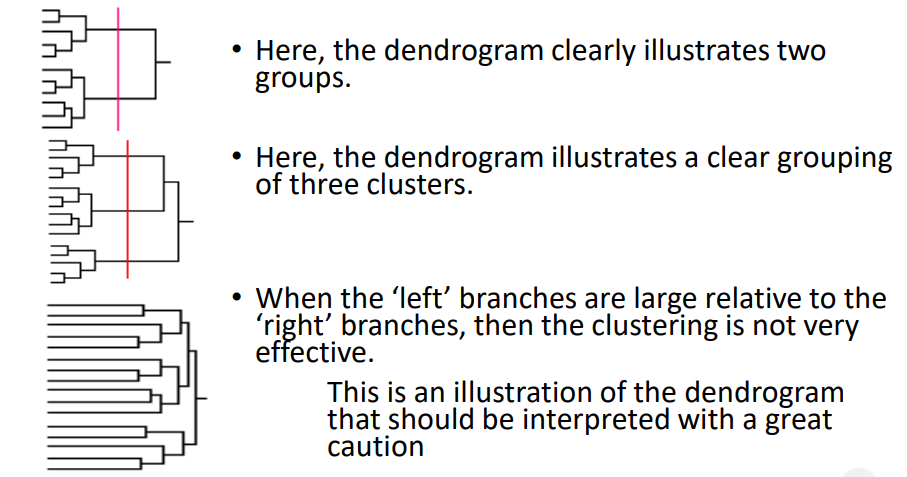
\includegraphics[width= \textwidth]{Images/Dendrograms.PNG}
    \caption{Interpreting a dendrogram}
    \label{fig:dendrogram}
\end{figure}
\smallskip
You should cut a tree when the gaps between the clusters is the largest.
\\\\
Interpretation of the clustering depends on the linkage method selected.
\subsubsection{Similarity}
There are many ways of measuring similarity between clusters the most common way is using Euclidean distance
\subsubsubsection{Euclidean Distance}
\begin{equation}
    d(x,y) = \sqrt{\sum_{i=1}^n (x_i - y_i)^2}
\end{equation}
\\\\
Euclidean distance is the standard measure for clustering.
\subsubsubsection{Squared Euclidean Distance}
\begin{equation}
    d(x,y) = \sum_{i=1}^n (x_i - y_i)^2
\end{equation}
\\\\
This helps to get dense clusters, if we were to plot the cluster in a multidimensional space, we would like them to be relatively dense aggregations of points, with small distance between points within clusters and big distances between clusters
\subsubsubsection{Cosine  similarity}
\begin{equation}
    sim(x,y) = \cos(\theta) = \frac{x\cdot y}{\lVert x \rVert\lVert y\rVert}
\end{equation}
\\\\
The more similar object the closer the points, Cosine is maximal for similar objects.
\subsubsubsection{Manhattan Block}
\begin{equation}
    d(x,y) = \lVert x-y \rVert = \sum_{i=1}^n \lVert x_i - y_i \rVert
\end{equation}
\\\\
The geometry has been used in regression analysis since the 18th century, and today is often referred to as LASSO.
\subsection{Cluster Analysis}
Possible problems with Euclidean and squared Euclidean distances is different scales for different variables, one way to get around this problem is to standardise the variables using the Z-score.
\\\\
Cluster analysis methods will always produce a grouping the groupings produceds by cluster analysis may ore may not be useful for classifying objects. There are many options for cluster analysis therefore we can mine the data trying different methods combining different distances and linkages to discover the structure in the data. 
\\\\
There are many example of successful application of cluster analysis to real problems a famous example, PRIZM system: In 1970s the company Claritas clustered neighbourhoods (U.S. zip codes) into forty different groups based on census information, such as population density, income, age, etc. This classification scheme, call PRIZM (Potential Rating Index for Zip Markets), has proven to be very useful in direct mail advertising, radio station formats, and decisions about where to locate stores.
\subsection{K-means: Non-hierarchical clustering}
This method differs from hierarchical clustering in many ways, the most obvious ways being 
\begin{itemize}
    \item There is no hierarchy, the data is partitioned instead
    \item You have to supply the number of clusters (k) into which you want to data to be grouped
\end{itemize}
This method is conceptually simple but computationally intensive
\begin{itemize}
    \item The cases are initially assigned randomly to the k clusters
    \item Cases are then moved around between clusters using an iterative method so that a classification is produced such that the clusters must be internally similar but externally dissimilar to the other clusters
    \item We stop when moving any more cases between clusters would make the clusters become more variable.
\end{itemize}
Cluster variability is measured with respect to their means for the classifying variables, hence the name k-means clustering. If more than one variable is used to define the clusters then the distances between clusters are measured in multi-dimensional space
\\\\
K-means is a relatively simple procedure, and consists of
choosing random k points that represent the distinct centres
of the k subsets, which are called centroids.
\begin{itemize}
    \item We then select, for each centroid, all the points closest to it
    \item This will create k different subsets.
    \item At this point, for each subset, we will re-calculate the centre
    \item We have again, k new centroids, and we repeat the steps above, selecting for each centroid, the new subsets of points closest to the centroids.
    \item  We continue this process until the centroids stop moving
\end{itemize}
For this technique to work, we need to be able to identify a metric that allows us to calculate the distance between points. This summarised as follows.
\begin{enumerate}
    \item Choose initial k-points, called centroids
    \item To each point in the data set, associate the closest centroid
    \item Calculate the new centre for the sets of points associated to a particular centroid
    \item Define the new centres to the new centroids
    \item Repeat steps 3 and 4 until the centroids stop moving
\end{enumerate}
\subsubsection{Silhouette}
Clustering results can be represented in a graphical form using silhouettes.
\\\\
The silhouette value for each point is a measure of how similar that point is to points in its own cluster, when compared to points in other clusters. The silhouette value for the  $i\;th$ point, $S_i$, is defined as
\begin{equation}
    S_i = \frac{b_i - a_i}{max(a_i,b_i)}
\end{equation}
Where $a_i$, is the average distance from the $i\;th$ point to the other points in the same cluster as $i$, and $b_i$ is the minimum average distance from the $i\;th$ point to points in a different cluster, minimised over clusters.
\\\\
The silhouette value ranges from -1 to +1, a high silhouette value for point $i$ indicates that this point is well-matched to its own cluster, and poorly-matched to neighboring clusters. If most points have a high silhouette value, then the clustering solution is appropriate. If many points have a low or negative silhouette value, then the clustering solution may have either too many or too few clusters. The silhouette clustering evaluation criterion can be used with any distance metric. The mean silhouette value can be used to estimate a quality of clustering.
\subsubsection{What to bear in mind}
It is important to notice that this method is extremely sensitive to the initial choice of random centroids, and that it may be a good idea to repeat the process for different initial choices. Also it is possible for some of the centroids not to be closest to any of the points ion the data-set reducing the number of subsets down from k.
\subsection{K Nearest Neighbour (KNN) Classifier}
This is a type of instance-based learning, or lazy learning, where the function is only approximated locally and all computation is deferred until classification. The KNN algorithm is among the simplest of all machine learning algorithms. The training examples are vectors in a multidimensional feature space each with a class label. The training phase of the algorithm consists only of storing the feature vectors and class labels of the training samples.  In the classification phase, k is a user-defined constant, and an unlabelled vector (a query or test point) is classified by assigning the label which is most frequent among the k training samples nearest to that query point.
\subsubsection{Algorithm summary}
\begin{itemize}
    \item A positive integer k is specified, along with a new sample
    \item We select the k entries in our database which are closest to the new sample
    \item We find the most common classification of these entries
    \item This is the classification we give the new sample
\end{itemize}
\subsubsection{Features of KNN}
KNN stores the entire training data-set which it uses as its representation, KNN does not learn any model and it makes predictions just-in-time by calculating the similarity between an input sample and each training instance.
\subsubsection{Pros and cons of KNN}
Pros
\begin{itemize}
    \item No assumptions about data — useful, for example, for nonlinear data
    \item Simple algorithm — to explain and understand/interpret
    \item High accuracy (relatively) — it is pretty high but not competitive in comparison to better supervised learning models
\end{itemize}
Cons
\begin{itemize}
    \item Computationally expensive —because the algorithm stores all of the training data
    \item High memory requirement
    \item Stores all (or almost all) of the training data
    \item Testing stage might be slow for large N
    \item Sensitive to irrelevant features and the scale of the data
\end{itemize}